\documentclass[12pt]{article}
\usepackage[table]{xcolor}
\usepackage[shortlabels]{enumitem}
\usepackage{tabularx,xltabular}
\usepackage{graphicx}
\usepackage{hyperref}
\usepackage{verbatim}
\usepackage{geometry}
\usepackage{ulem}
\usepackage[official]{eurosym}
\usepackage{tikz}
\usetikzlibrary{arrows,backgrounds,calc,decorations.markings,patterns,3d}
\usepackage{pgfplots}
\pgfplotsset{compat = newest}
\usetikzlibrary{fit}
\newcommand\addvmargin[1]{
\usetikzlibrary{arrows}
\node[fit=(current bounding box),inner ysep=#1,inner xsep=0]{};}
\usepackage{cancel}
\usepackage{fontspec}
\usepackage{array}  
\geometry{a4paper, top=2cm, left=2cm, right=2cm, bottom=2cm, headsep=1cm}
\usepackage{tabu}
\usepackage{pst-node}
\usepackage{colortbl}
\usepackage{array}
\usepackage{german}
\setlength\parindent{0pt}
\newcolumntype{?}{!{\vrule width 1pt}}
\usepackage{makecell}
\renewcommand{\arraystretch}{2.5}
\usepackage{pbox}
\usepackage{amssymb}
\usepackage{amsmath}
\usepackage{booktabs}
\newcolumntype{L}[1]{>{\raggedright\let\newline\\\arraybackslash\hspace{0pt}}m{#1}}
\newcolumntype{C}[1]{>{\centering\let\newline\\\arraybackslash\hspace{0pt}}m{#1}}
\newcolumntype{R}[1]{>{\raggedleft\let\newline\\\arraybackslash\hspace{0pt}}m{#1}}
\begin{document}
\rightline{Datum: 08.06.2023}
\centerline{{\Large Tägliche Übungen}} 
\vspace{1cm}
\noindent \\


\begin{xltabular}{\textwidth}{|C{0.75cm}|X|C{0.75cm}|X|}
\arrayrulecolor{black}\hline
a)&$\begin{aligned}
 x=&-8~ \rightarrow ~ 3 + 3 \cdot x=?
\end{aligned}$
&
b)&$\begin{aligned}
 x=&7~ \rightarrow ~ 2 \cdot x + 5=?
\end{aligned}$
\\\hline
c)&$\begin{aligned}
 b=&11~ \rightarrow ~ 5 \cdot b - 5=?
\end{aligned}$
&
d)&$\begin{aligned}
 b=&6~ \rightarrow ~ 4 \cdot b + 5 \cdot b=?
\end{aligned}$
\\\hline
e)&$y+25 = 37$
&
f)&$a+33 = 40$
\\\hline
g)&$x-18 = 14$
&
h)&$a+21 = 36$
\\\hline
i)&$b+45 = 14$
&
j)&$x+27 = 44$
\\\hline
k)&$x+18 = 16$
&
l)&$b-38 = 17$
\\\hline
m)&$y-9 = 9$
&
n)&$a-15 = 21$
\\\hline
o)&$a+6 = 27$
&
p)&$b-31 = 50$
\\\hline
q)&$x+43 = 41$
&
r)&$a-7 = 38$
\\\hline
s)&$a+47 = 8$
&
t)&$y-23 = 5$
\\\hline
u)&$a+6 = 25$
&
v)&$x-25 = 1$
\\\hline
w)&$b-40 = 10$
&
x)&$b+23 = 26$
\\\hline
y)&$y-34 = 41$
&
z)&$b+37 = 38$
\\\hline
\end{xltabular}
\vspace{0.5cm}
\newpage
\rightline{Datum: 08.06.2023}
\centerline{{\large Lösungen Tägliche Übungen}} 
\vspace{0.5cm}

\begin{xltabular}{\textwidth}{|C{0.75cm}|X|C{0.75cm}|X|}
\arrayrulecolor{black}\hline
a)&$\begin{aligned}
\textcolor{red}{x=-8} & \rightarrow\\
3 + 3 \cdot x=&3 + 3 \cdot \textcolor{red}{(-8)}=-21\\
\end{aligned}$
&
b)&$\begin{aligned}
\textcolor{red}{x=7} & \rightarrow\\
2 \cdot x + 5=&2 \cdot \textcolor{red}{7} + 5=19\\
\end{aligned}$
\\\hline
c)&$\begin{aligned}
\textcolor{red}{b=11} & \rightarrow\\
5 \cdot b - 5=&5 \cdot \textcolor{red}{11} - 5=50\\
\end{aligned}$
&
d)&$\begin{aligned}
\textcolor{red}{b=6} & \rightarrow\\
4 \cdot b + 5 \cdot b=&4 \cdot \textcolor{red}{6} + 5 \cdot \textcolor{red}{6}=54\\
\end{aligned}$
\\\hline
e)&\begingroup\setlength{\jot}{-0.03cm}
\tikzstyle{background grid}=[draw, black!15,step=.5cm]
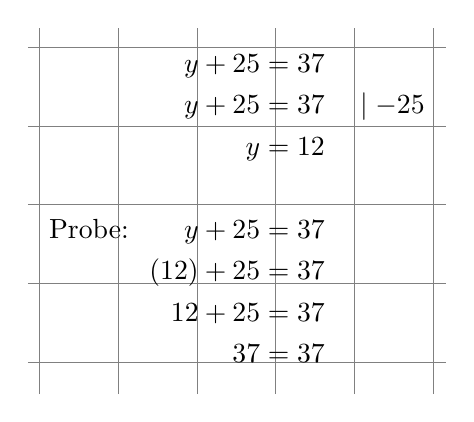
\begin{tikzpicture}[show background grid]
\node[below right] at (0,0.1) {
$\begin{aligned}
y+25  &= 37& &  \\
y + 25 &=37& & \mid - 25\\
y &=12& & 
\\
\\
\mbox{Probe:}\qquad y+25  &= 37& &  \\
\left(12\right)+25  &= 37& &  \\
12+25 &=37& &  \\
37 &=37& &  \\
\end{aligned}$};
\end{tikzpicture}
\endgroup
&
f)&\begingroup\setlength{\jot}{-0.03cm}
\tikzstyle{background grid}=[draw, black!15,step=.5cm]
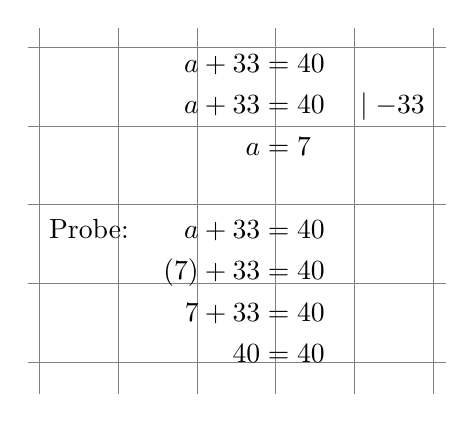
\begin{tikzpicture}[show background grid]
\node[below right] at (0,0.1) {
$\begin{aligned}
a+33  &= 40& &  \\
a + 33 &=40& & \mid - 33\\
a &=7& & 
\\
\\
\mbox{Probe:}\qquad a+33  &= 40& &  \\
\left(7\right)+33  &= 40& &  \\
7+33 &=40& &  \\
40 &=40& &  \\
\end{aligned}$};
\end{tikzpicture}
\endgroup
\\\hline
g)&\begingroup\setlength{\jot}{-0.03cm}
\tikzstyle{background grid}=[draw, black!15,step=.5cm]
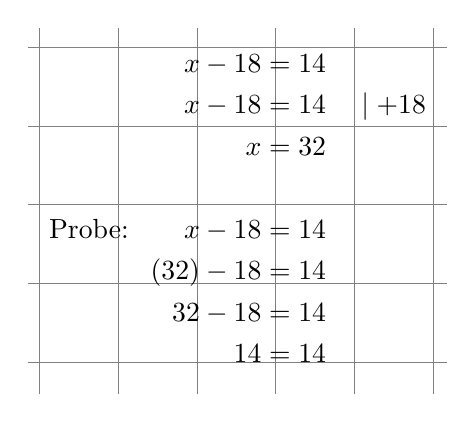
\begin{tikzpicture}[show background grid]
\node[below right] at (0,0.1) {
$\begin{aligned}
x-18  &= 14& &  \\
x - 18 &=14& & \mid + 18\\
x &=32& & 
\\
\\
\mbox{Probe:}\qquad x-18  &= 14& &  \\
\left(32\right)-18  &= 14& &  \\
32-18 &=14& &  \\
14 &=14& &  \\
\end{aligned}$};
\end{tikzpicture}
\endgroup
&
h)&\begingroup\setlength{\jot}{-0.03cm}
\tikzstyle{background grid}=[draw, black!15,step=.5cm]
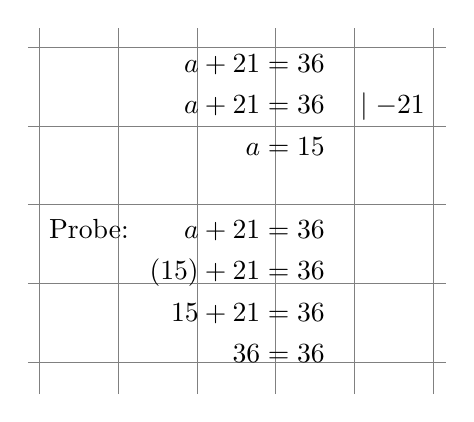
\begin{tikzpicture}[show background grid]
\node[below right] at (0,0.1) {
$\begin{aligned}
a+21  &= 36& &  \\
a + 21 &=36& & \mid - 21\\
a &=15& & 
\\
\\
\mbox{Probe:}\qquad a+21  &= 36& &  \\
\left(15\right)+21  &= 36& &  \\
15+21 &=36& &  \\
36 &=36& &  \\
\end{aligned}$};
\end{tikzpicture}
\endgroup
\\\hline
i)&\begingroup\setlength{\jot}{-0.03cm}
\tikzstyle{background grid}=[draw, black!15,step=.5cm]
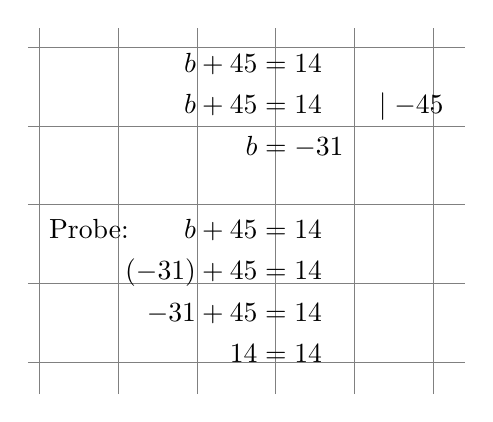
\begin{tikzpicture}[show background grid]
\node[below right] at (0,0.1) {
$\begin{aligned}
b+45  &= 14& &  \\
b + 45 &=14& & \mid - 45\\
b &=-31& & 
\\
\\
\mbox{Probe:}\qquad b+45  &= 14& &  \\
\left(-31\right)+45  &= 14& &  \\
-31+45 &=14& &  \\
14 &=14& &  \\
\end{aligned}$};
\end{tikzpicture}
\endgroup
&
j)&\begingroup\setlength{\jot}{-0.03cm}
\tikzstyle{background grid}=[draw, black!15,step=.5cm]
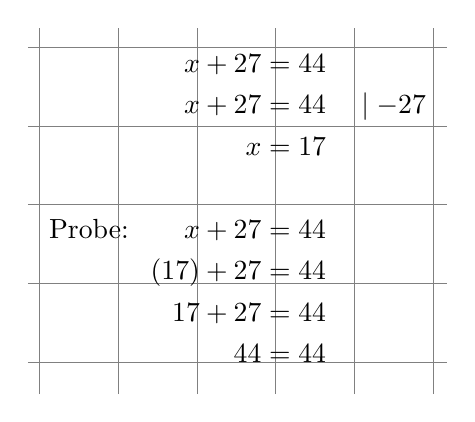
\begin{tikzpicture}[show background grid]
\node[below right] at (0,0.1) {
$\begin{aligned}
x+27  &= 44& &  \\
x + 27 &=44& & \mid - 27\\
x &=17& & 
\\
\\
\mbox{Probe:}\qquad x+27  &= 44& &  \\
\left(17\right)+27  &= 44& &  \\
17+27 &=44& &  \\
44 &=44& &  \\
\end{aligned}$};
\end{tikzpicture}
\endgroup
\\\hline
k)&\begingroup\setlength{\jot}{-0.03cm}
\tikzstyle{background grid}=[draw, black!15,step=.5cm]
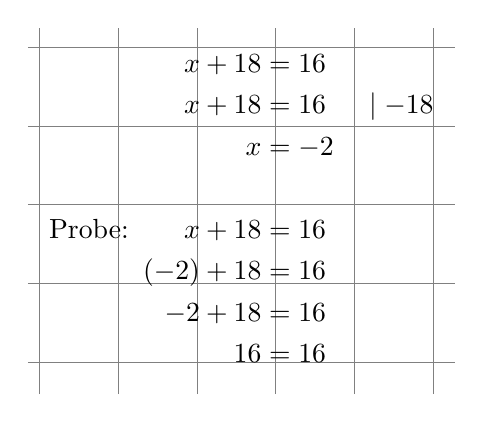
\begin{tikzpicture}[show background grid]
\node[below right] at (0,0.1) {
$\begin{aligned}
x+18  &= 16& &  \\
x + 18 &=16& & \mid - 18\\
x &=-2& & 
\\
\\
\mbox{Probe:}\qquad x+18  &= 16& &  \\
\left(-2\right)+18  &= 16& &  \\
-2+18 &=16& &  \\
16 &=16& &  \\
\end{aligned}$};
\end{tikzpicture}
\endgroup
&
l)&\begingroup\setlength{\jot}{-0.03cm}
\tikzstyle{background grid}=[draw, black!15,step=.5cm]
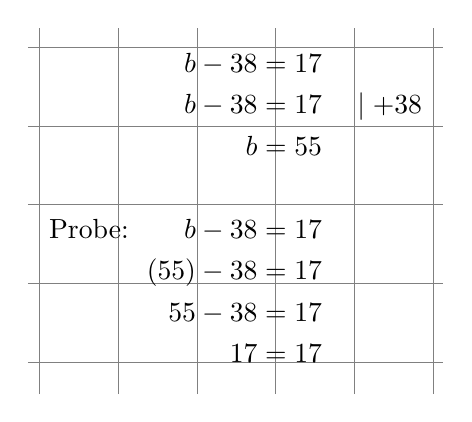
\begin{tikzpicture}[show background grid]
\node[below right] at (0,0.1) {
$\begin{aligned}
b-38  &= 17& &  \\
b - 38 &=17& & \mid + 38\\
b &=55& & 
\\
\\
\mbox{Probe:}\qquad b-38  &= 17& &  \\
\left(55\right)-38  &= 17& &  \\
55-38 &=17& &  \\
17 &=17& &  \\
\end{aligned}$};
\end{tikzpicture}
\endgroup
\\\hline
m)&\begingroup\setlength{\jot}{-0.03cm}
\tikzstyle{background grid}=[draw, black!15,step=.5cm]
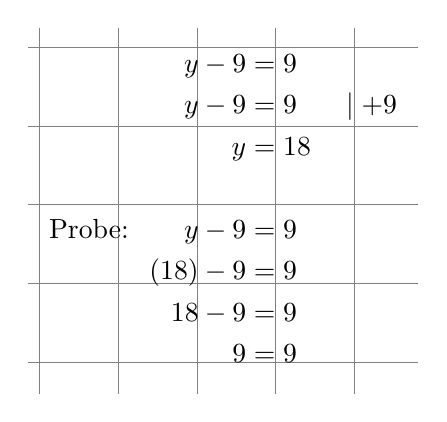
\begin{tikzpicture}[show background grid]
\node[below right] at (0,0.1) {
$\begin{aligned}
y-9  &= 9& &  \\
y - 9 &=9& & \mid + 9\\
y &=18& & 
\\
\\
\mbox{Probe:}\qquad y-9  &= 9& &  \\
\left(18\right)-9  &= 9& &  \\
18-9 &=9& &  \\
9 &=9& &  \\
\end{aligned}$};
\end{tikzpicture}
\endgroup
&
n)&\begingroup\setlength{\jot}{-0.03cm}
\tikzstyle{background grid}=[draw, black!15,step=.5cm]
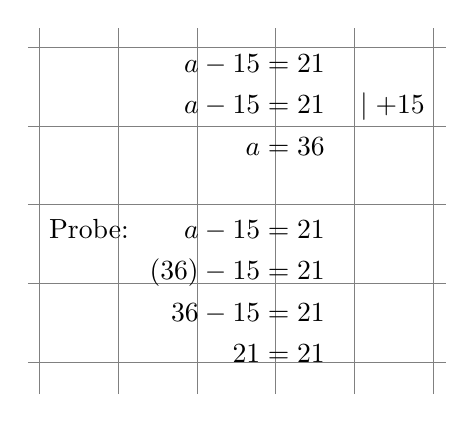
\begin{tikzpicture}[show background grid]
\node[below right] at (0,0.1) {
$\begin{aligned}
a-15  &= 21& &  \\
a - 15 &=21& & \mid + 15\\
a &=36& & 
\\
\\
\mbox{Probe:}\qquad a-15  &= 21& &  \\
\left(36\right)-15  &= 21& &  \\
36-15 &=21& &  \\
21 &=21& &  \\
\end{aligned}$};
\end{tikzpicture}
\endgroup
\\\hline
o)&\begingroup\setlength{\jot}{-0.03cm}
\tikzstyle{background grid}=[draw, black!15,step=.5cm]
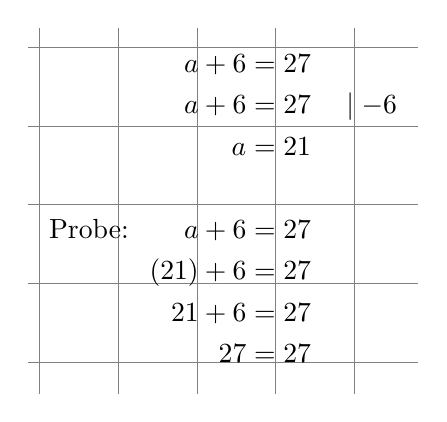
\begin{tikzpicture}[show background grid]
\node[below right] at (0,0.1) {
$\begin{aligned}
a+6  &= 27& &  \\
a + 6 &=27& & \mid - 6\\
a &=21& & 
\\
\\
\mbox{Probe:}\qquad a+6  &= 27& &  \\
\left(21\right)+6  &= 27& &  \\
21+6 &=27& &  \\
27 &=27& &  \\
\end{aligned}$};
\end{tikzpicture}
\endgroup
&
p)&\begingroup\setlength{\jot}{-0.03cm}
\tikzstyle{background grid}=[draw, black!15,step=.5cm]
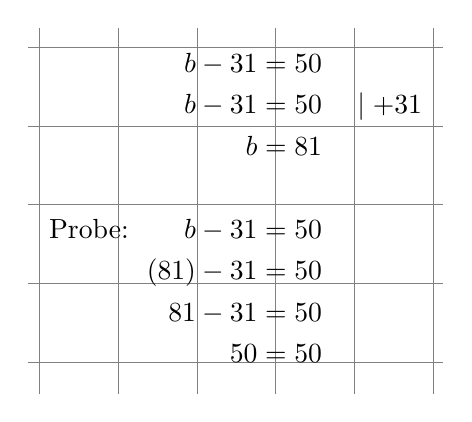
\begin{tikzpicture}[show background grid]
\node[below right] at (0,0.1) {
$\begin{aligned}
b-31  &= 50& &  \\
b - 31 &=50& & \mid + 31\\
b &=81& & 
\\
\\
\mbox{Probe:}\qquad b-31  &= 50& &  \\
\left(81\right)-31  &= 50& &  \\
81-31 &=50& &  \\
50 &=50& &  \\
\end{aligned}$};
\end{tikzpicture}
\endgroup
\\\hline
q)&\begingroup\setlength{\jot}{-0.03cm}
\tikzstyle{background grid}=[draw, black!15,step=.5cm]
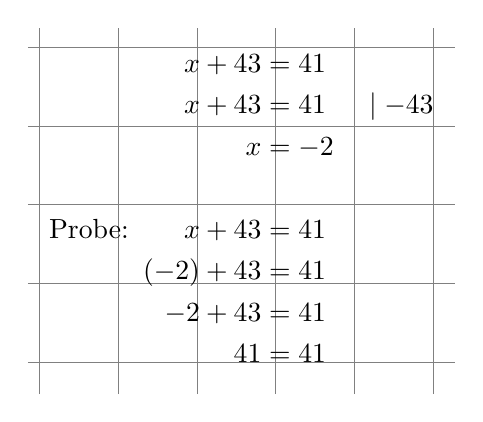
\begin{tikzpicture}[show background grid]
\node[below right] at (0,0.1) {
$\begin{aligned}
x+43  &= 41& &  \\
x + 43 &=41& & \mid - 43\\
x &=-2& & 
\\
\\
\mbox{Probe:}\qquad x+43  &= 41& &  \\
\left(-2\right)+43  &= 41& &  \\
-2+43 &=41& &  \\
41 &=41& &  \\
\end{aligned}$};
\end{tikzpicture}
\endgroup
&
r)&\begingroup\setlength{\jot}{-0.03cm}
\tikzstyle{background grid}=[draw, black!15,step=.5cm]
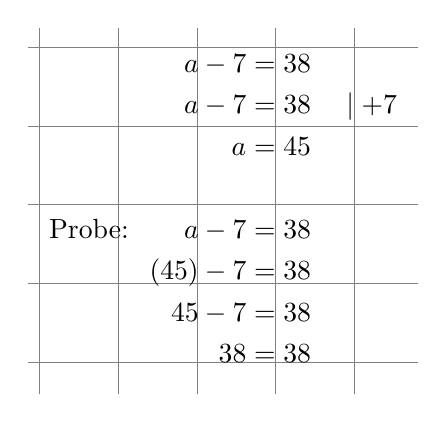
\begin{tikzpicture}[show background grid]
\node[below right] at (0,0.1) {
$\begin{aligned}
a-7  &= 38& &  \\
a - 7 &=38& & \mid + 7\\
a &=45& & 
\\
\\
\mbox{Probe:}\qquad a-7  &= 38& &  \\
\left(45\right)-7  &= 38& &  \\
45-7 &=38& &  \\
38 &=38& &  \\
\end{aligned}$};
\end{tikzpicture}
\endgroup
\\\hline
s)&\begingroup\setlength{\jot}{-0.03cm}
\tikzstyle{background grid}=[draw, black!15,step=.5cm]
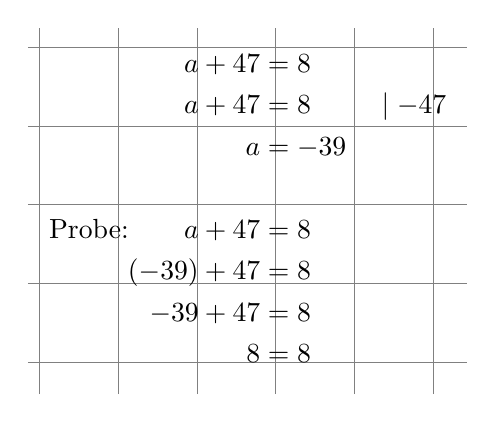
\begin{tikzpicture}[show background grid]
\node[below right] at (0,0.1) {
$\begin{aligned}
a+47  &= 8& &  \\
a + 47 &=8& & \mid - 47\\
a &=-39& & 
\\
\\
\mbox{Probe:}\qquad a+47  &= 8& &  \\
\left(-39\right)+47  &= 8& &  \\
-39+47 &=8& &  \\
8 &=8& &  \\
\end{aligned}$};
\end{tikzpicture}
\endgroup
&
t)&\begingroup\setlength{\jot}{-0.03cm}
\tikzstyle{background grid}=[draw, black!15,step=.5cm]
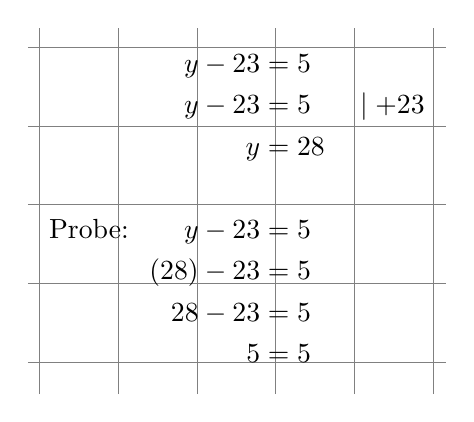
\begin{tikzpicture}[show background grid]
\node[below right] at (0,0.1) {
$\begin{aligned}
y-23  &= 5& &  \\
y - 23 &=5& & \mid + 23\\
y &=28& & 
\\
\\
\mbox{Probe:}\qquad y-23  &= 5& &  \\
\left(28\right)-23  &= 5& &  \\
28-23 &=5& &  \\
5 &=5& &  \\
\end{aligned}$};
\end{tikzpicture}
\endgroup
\\\hline
u)&\begingroup\setlength{\jot}{-0.03cm}
\tikzstyle{background grid}=[draw, black!15,step=.5cm]
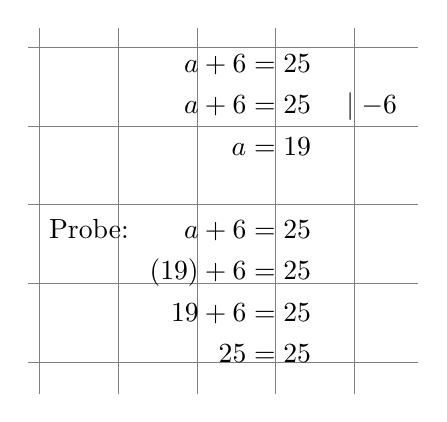
\begin{tikzpicture}[show background grid]
\node[below right] at (0,0.1) {
$\begin{aligned}
a+6  &= 25& &  \\
a + 6 &=25& & \mid - 6\\
a &=19& & 
\\
\\
\mbox{Probe:}\qquad a+6  &= 25& &  \\
\left(19\right)+6  &= 25& &  \\
19+6 &=25& &  \\
25 &=25& &  \\
\end{aligned}$};
\end{tikzpicture}
\endgroup
&
v)&\begingroup\setlength{\jot}{-0.03cm}
\tikzstyle{background grid}=[draw, black!15,step=.5cm]
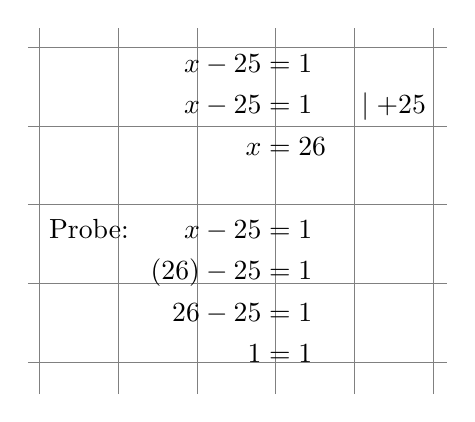
\begin{tikzpicture}[show background grid]
\node[below right] at (0,0.1) {
$\begin{aligned}
x-25  &= 1& &  \\
x - 25 &=1& & \mid + 25\\
x &=26& & 
\\
\\
\mbox{Probe:}\qquad x-25  &= 1& &  \\
\left(26\right)-25  &= 1& &  \\
26-25 &=1& &  \\
1 &=1& &  \\
\end{aligned}$};
\end{tikzpicture}
\endgroup
\\\hline
w)&\begingroup\setlength{\jot}{-0.03cm}
\tikzstyle{background grid}=[draw, black!15,step=.5cm]
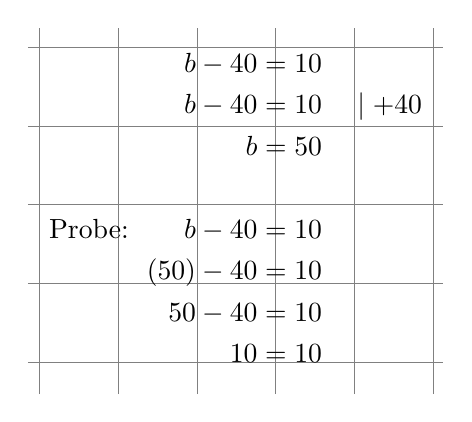
\begin{tikzpicture}[show background grid]
\node[below right] at (0,0.1) {
$\begin{aligned}
b-40  &= 10& &  \\
b - 40 &=10& & \mid + 40\\
b &=50& & 
\\
\\
\mbox{Probe:}\qquad b-40  &= 10& &  \\
\left(50\right)-40  &= 10& &  \\
50-40 &=10& &  \\
10 &=10& &  \\
\end{aligned}$};
\end{tikzpicture}
\endgroup
&
x)&\begingroup\setlength{\jot}{-0.03cm}
\tikzstyle{background grid}=[draw, black!15,step=.5cm]
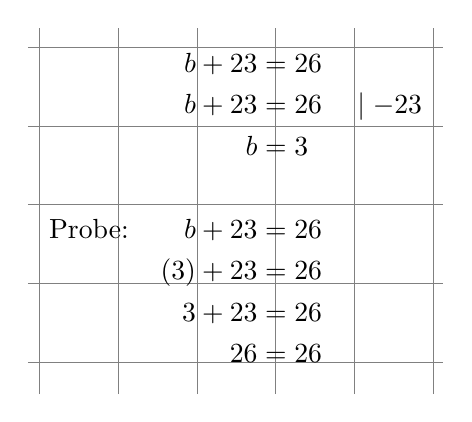
\begin{tikzpicture}[show background grid]
\node[below right] at (0,0.1) {
$\begin{aligned}
b+23  &= 26& &  \\
b + 23 &=26& & \mid - 23\\
b &=3& & 
\\
\\
\mbox{Probe:}\qquad b+23  &= 26& &  \\
\left(3\right)+23  &= 26& &  \\
3+23 &=26& &  \\
26 &=26& &  \\
\end{aligned}$};
\end{tikzpicture}
\endgroup
\\\hline
y)&\begingroup\setlength{\jot}{-0.03cm}
\tikzstyle{background grid}=[draw, black!15,step=.5cm]
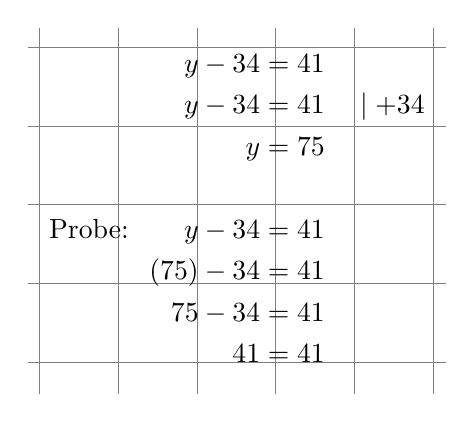
\begin{tikzpicture}[show background grid]
\node[below right] at (0,0.1) {
$\begin{aligned}
y-34  &= 41& &  \\
y - 34 &=41& & \mid + 34\\
y &=75& & 
\\
\\
\mbox{Probe:}\qquad y-34  &= 41& &  \\
\left(75\right)-34  &= 41& &  \\
75-34 &=41& &  \\
41 &=41& &  \\
\end{aligned}$};
\end{tikzpicture}
\endgroup
&
z)&\begingroup\setlength{\jot}{-0.03cm}
\tikzstyle{background grid}=[draw, black!15,step=.5cm]
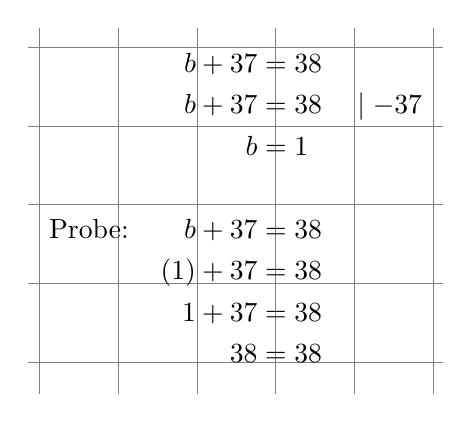
\begin{tikzpicture}[show background grid]
\node[below right] at (0,0.1) {
$\begin{aligned}
b+37  &= 38& &  \\
b + 37 &=38& & \mid - 37\\
b &=1& & 
\\
\\
\mbox{Probe:}\qquad b+37  &= 38& &  \\
\left(1\right)+37  &= 38& &  \\
1+37 &=38& &  \\
38 &=38& &  \\
\end{aligned}$};
\end{tikzpicture}
\endgroup
\\\hline
\end{xltabular}
\vspace{0.5cm}
\end{document}